\subsection{Présentation des projets}

A présent, nous allons analyser la manière de visualiser les objets patrimoniaux de trois projets utilisant l'intelligence artificielle pour réaliser de la reconnaissance automatique de similarités comme le fait l'application AIKON afin de mieux cerner les besoins nécessaires.

\begin{itemize}
	\item Le projet \textit{Visual Contagion} mené par la faculté des lettres de Genève a mis en place l'outil \textit{Explore}. Ce dernier sert à regrouper les images similaires en cluster. Le but de ce projet est d'étudier la circulation d'images de 1890 aux débuts d'internet à l'échelle mondiale. En effet, certaines ont davantage circulé que d'autres car elles ont été reproduites, copiés, imitées et pastichées. L'étude de ces images nous permet de nous questionner sur les raisons du succès de certaines d'entre-elles tout en saisissant comment leur circulation a contribué à la mondialisation de la culture. Le projet se questionne également sur les questions de domination symbolique de nation ou de culture en particulier à certains moments de l'histoire\footcite{HomeVisualContagions}.
	\item \textit{ONiT Explorer} est une plateforme dont le but est d'explorer une collection d'image tirées de récits de voyage dans l'Empire ottoman\footcite{ONiTExplorer}.
	\item \textit{iArt} est un moteur de recherche en histoire et histoire de l'art destinée à la recherche de similarités pour les chercheurs\footcite{IART}.
\end{itemize}

Pour étudier ces différents projets nous allons nous appuyer sur les critères que nous avons vu précédemment. 

\subsection{Analyse des interfaces}

\subsubsection{Les interfaces et leurs différentes vues}

Ce qui attire notre attention lorsque nous arrivons pour la première fois sur une plateforme est l'interface. En général, cette dernière est composée de plusieurs pages dont le nombre diffèrent en fonction des fonctionnalités et des différentes vues présentes. 

Dans les trois projets, il est possible d'appliquer l'analyse de Shneiderman\footcite{shneidermanEyesHaveIt} concernant la décomposition d'une \textit{generous interface}.

L'outil \textit{Explore} du projet \textit{Visual Contagion} est divisé en deux grandes parties. D'un côté, il y a une interface pour rechercher une image en particulier dans le corpus et une autre pour explorer les images similaires dans le corpus. Lorsque nous choisissons la deuxième option, nous arrivons sur la \textit{vue d'ensemble} où les images sont organisées en \textit{clusters} affichés de manière horizontale. Cette manière d'organiser l'application est propice à la découverte par sérendipité car le visiteur déambule à travers les différents clusters comme s'il était dans un musée ou une bibliothèque. Il n'est pas obligé d'avoir une idée précise en tête ou de connaître parfaitement le corpus. 

\begin{figure}[H]
	\centering
	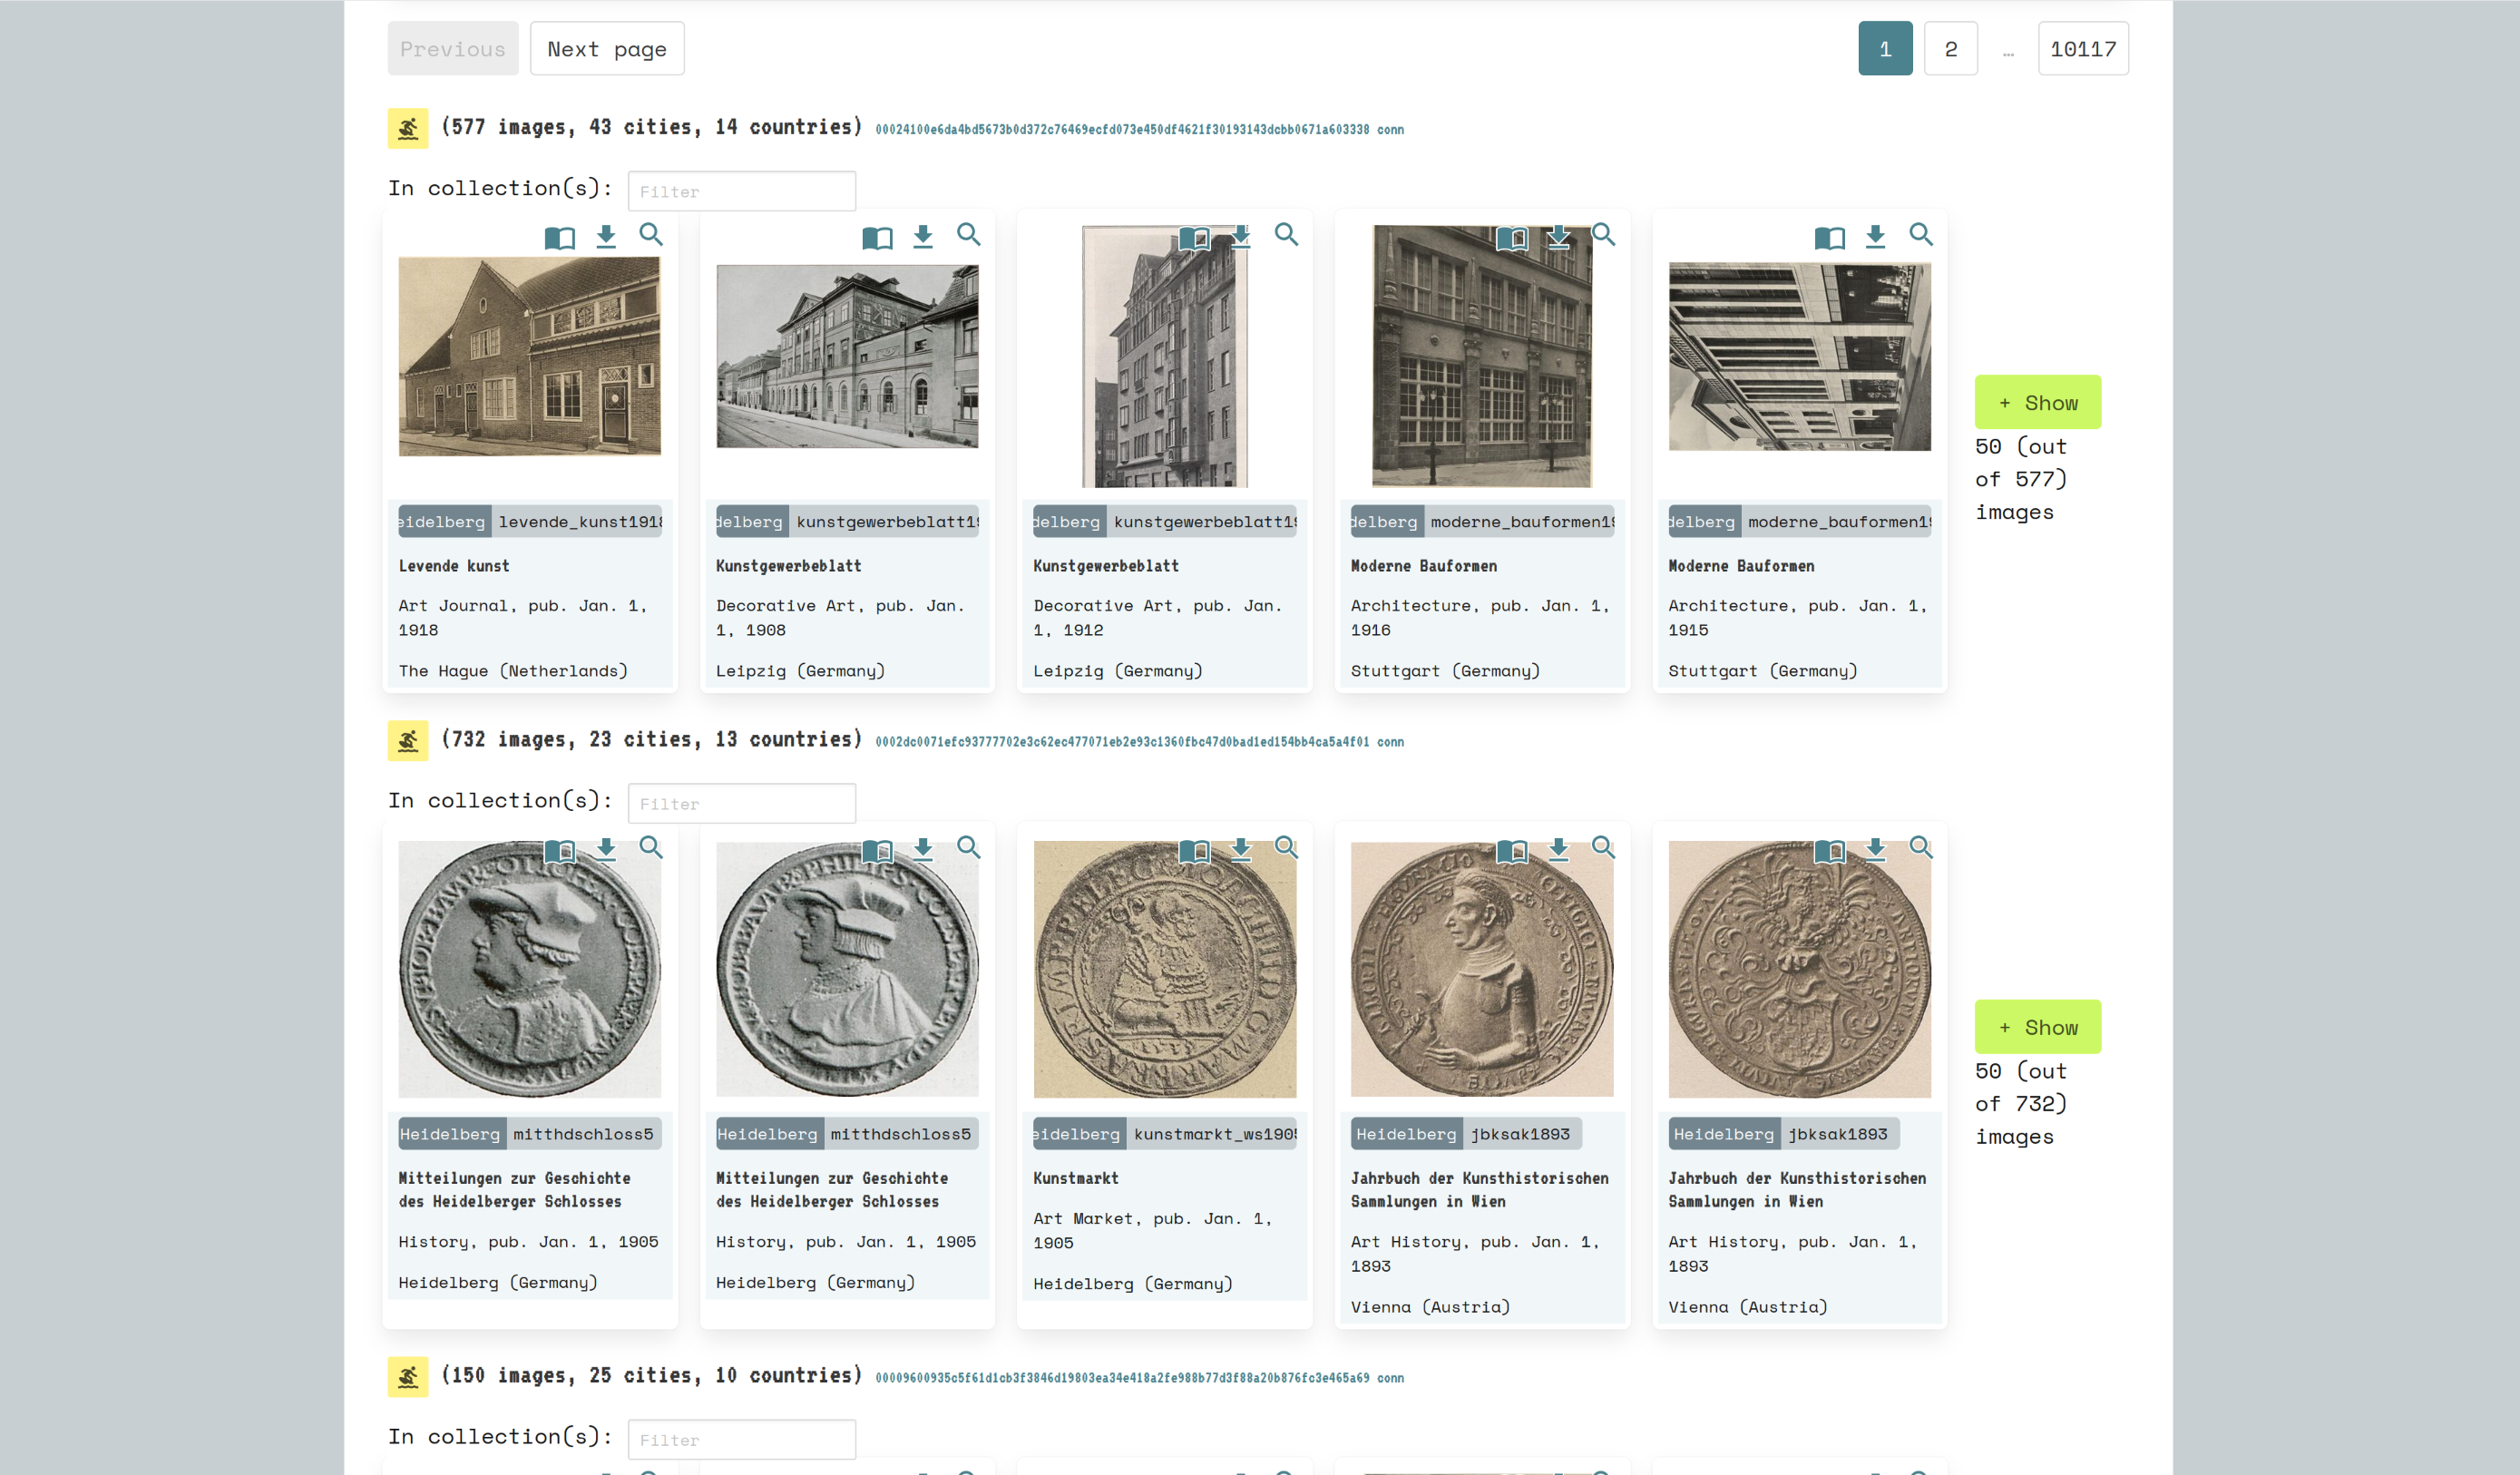
\includegraphics[width=0.8\textwidth]{images/visual_contagion_1.png}
	\caption{Capture d'écran de la \textit{vue d'ensemble} de différents \textit{clusters} sur la plateforme \textit{Explore}}
	\label{fig:explore_1}
\end{figure}

Quand nous utilisons le bouton \textit{+ Show}, toutes les images du \textit{cluster} s'affichent sous la forme d'une mosaïque. Si nous cliquons sur l'identifiant du \textit{cluster} en haut de celui-ci pour obtenir un \textit{sous-ensemble}, toutes les images le composant apparaissent sur une nouvelle page. Il existe une fonctionnalité nommée \textit{cluster-surf} qui permet d'afficher une visualisation chrono-cartographique où sont disposées toutes les images du \textit{cluster}. 

\begin{figure}[H]
	\centering
	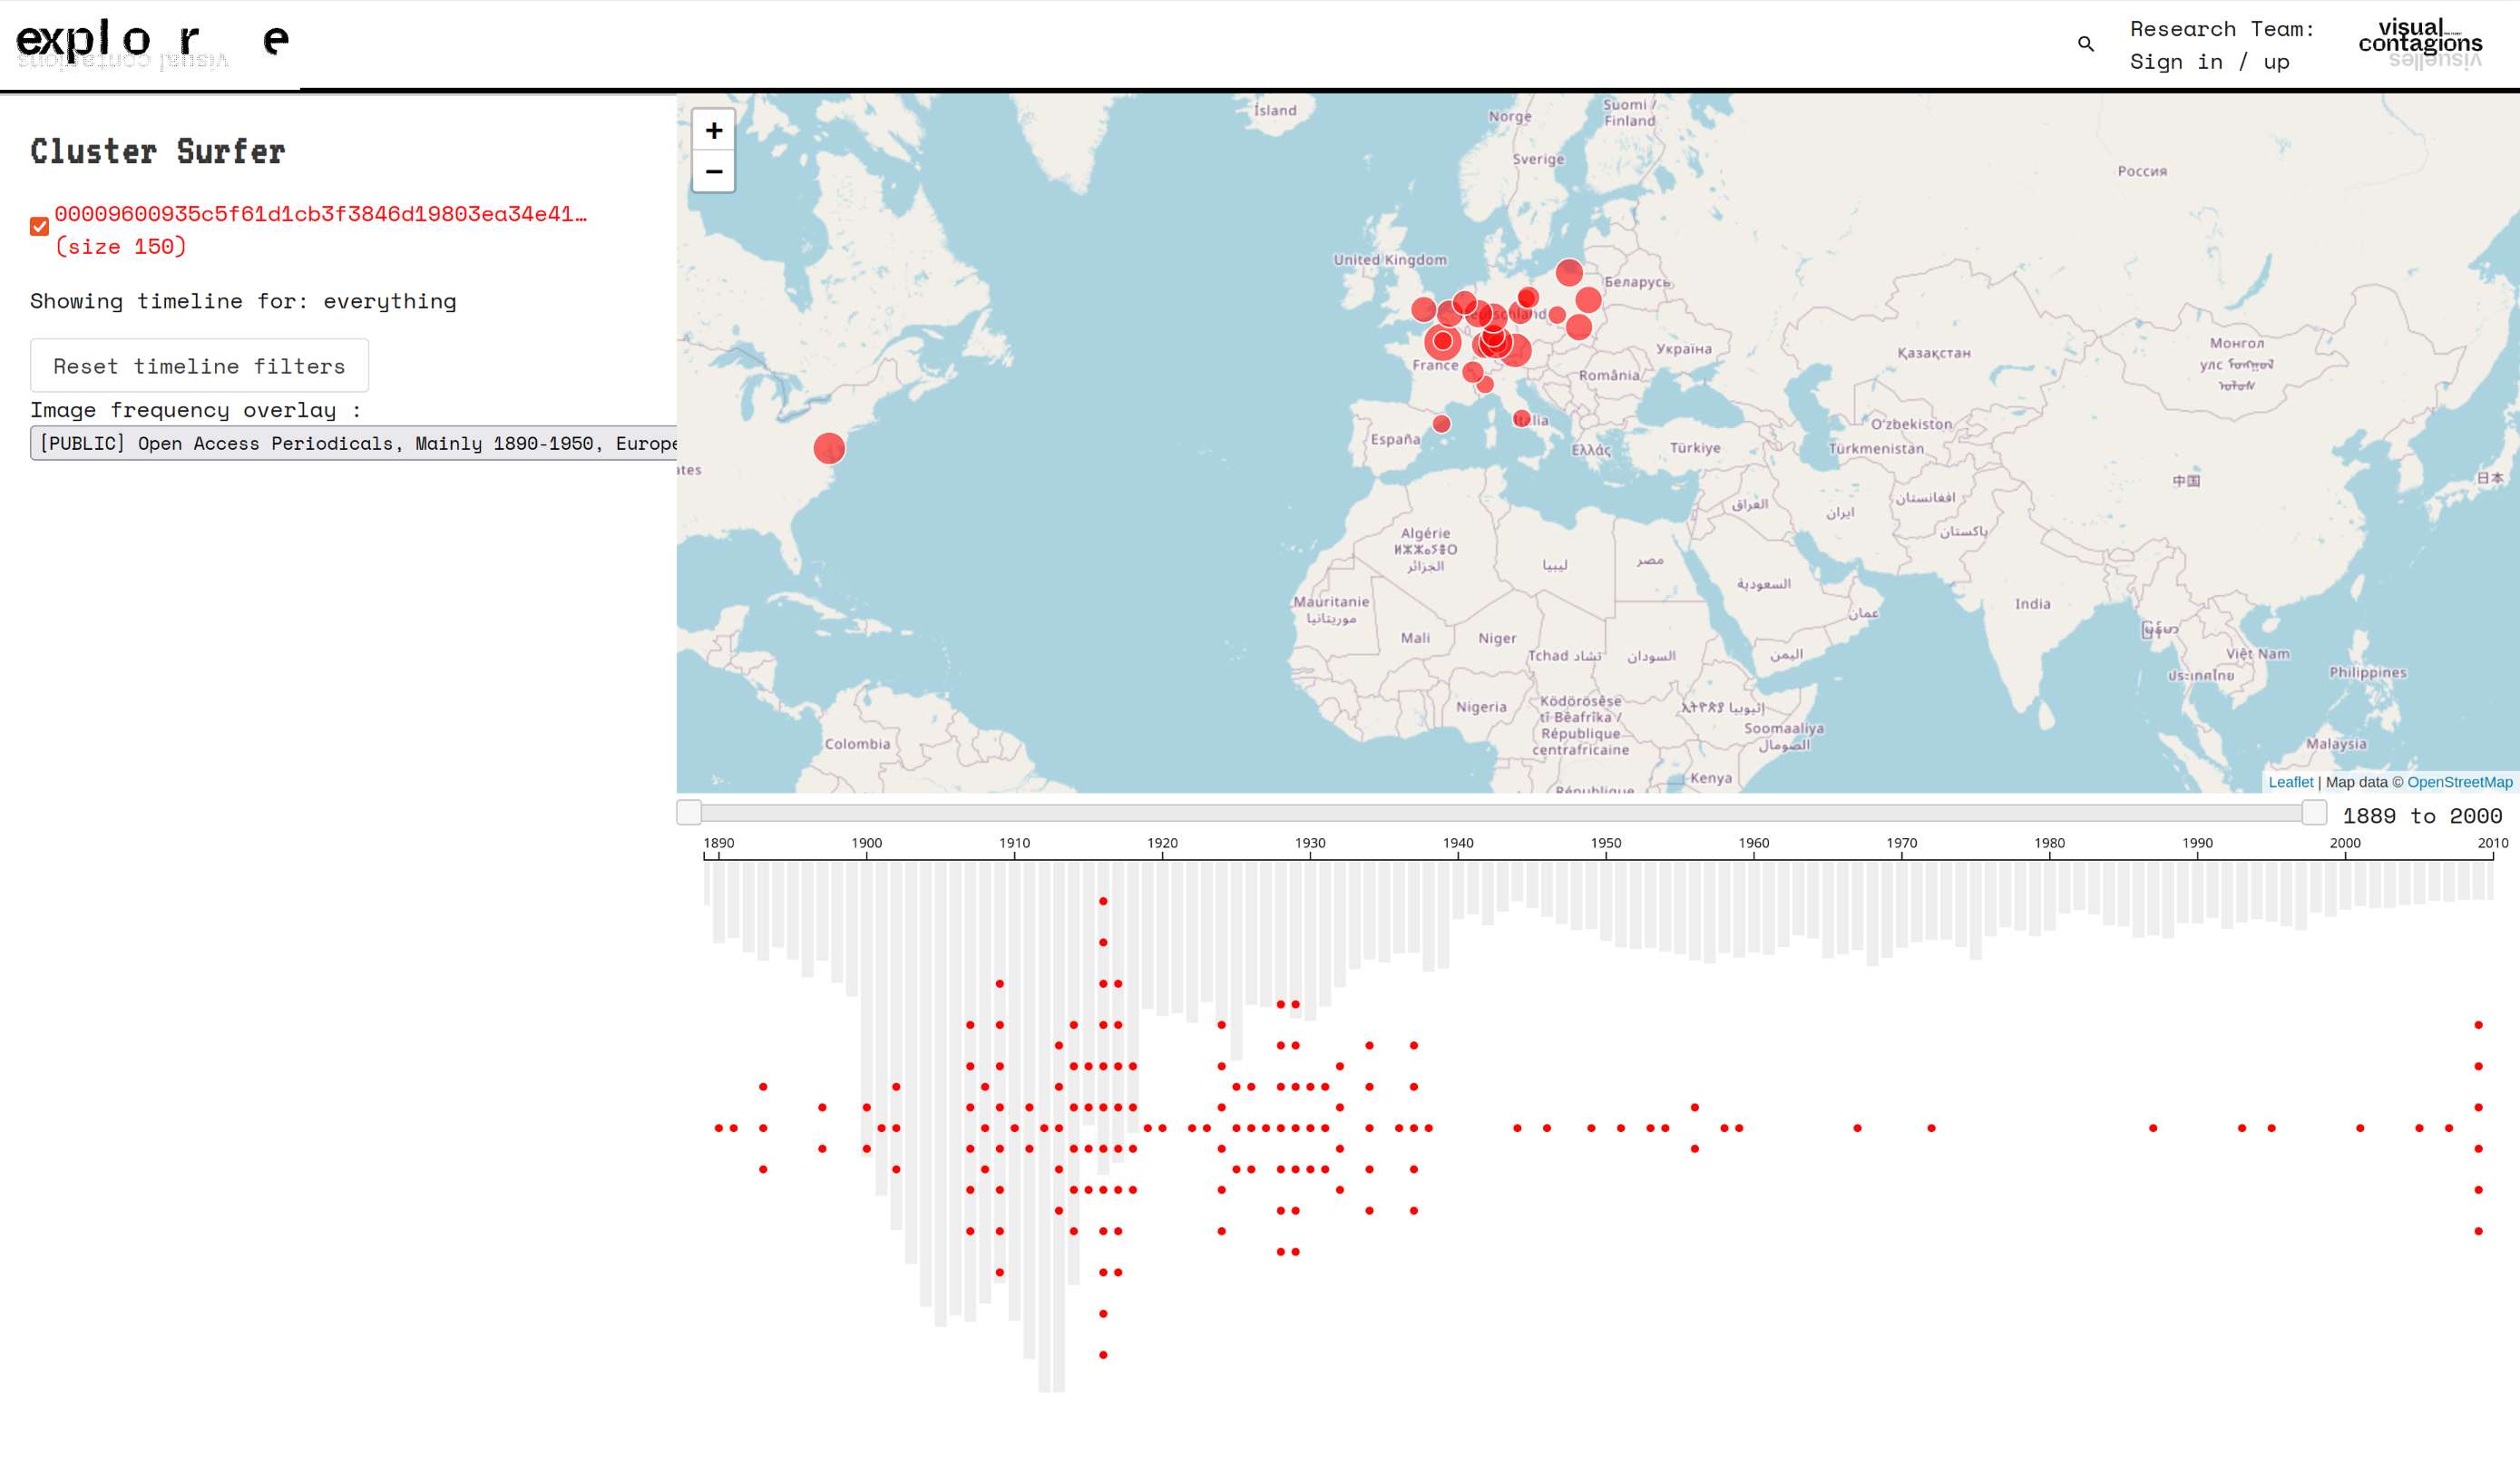
\includegraphics[width=0.8\textwidth]{images/visual_contagion_2.png}
	\caption{La fonctionnalité \textit{cluster-surfer} sur la plateforme \textit{Explore}}
	\label{fig:explore_2}
\end{figure}

Pour finir, il est possible de montrer le \textit{détail} pour voir les métadonnées ainsi que les liens vers les différents \textit{clusters} dans lesquels l'objet se situe. 

Pour la plateforme \textit{iArt}, lorsque nous faisons une recherche par mot-clé ou aléatoire, les images s'affichent en \textit{vue d'ensemble} sous la forme d'une mosaïque. Si nous utilisons la fonctionnalité \textit{Use 2D canvas view} dans \textit{Result view}, elles s'affichent en \textit{sous-ensemble} sous forme de \textit{clusters} éloignés dans l'espace. Si nous cliquons sur l'une d'entre-elles pour afficher le \textit{détail}, une fenêtre pop-up apparaît avec l'image, ses métadonnées et des \textit{tags}.

\begin{figure}[H]
	\centering
	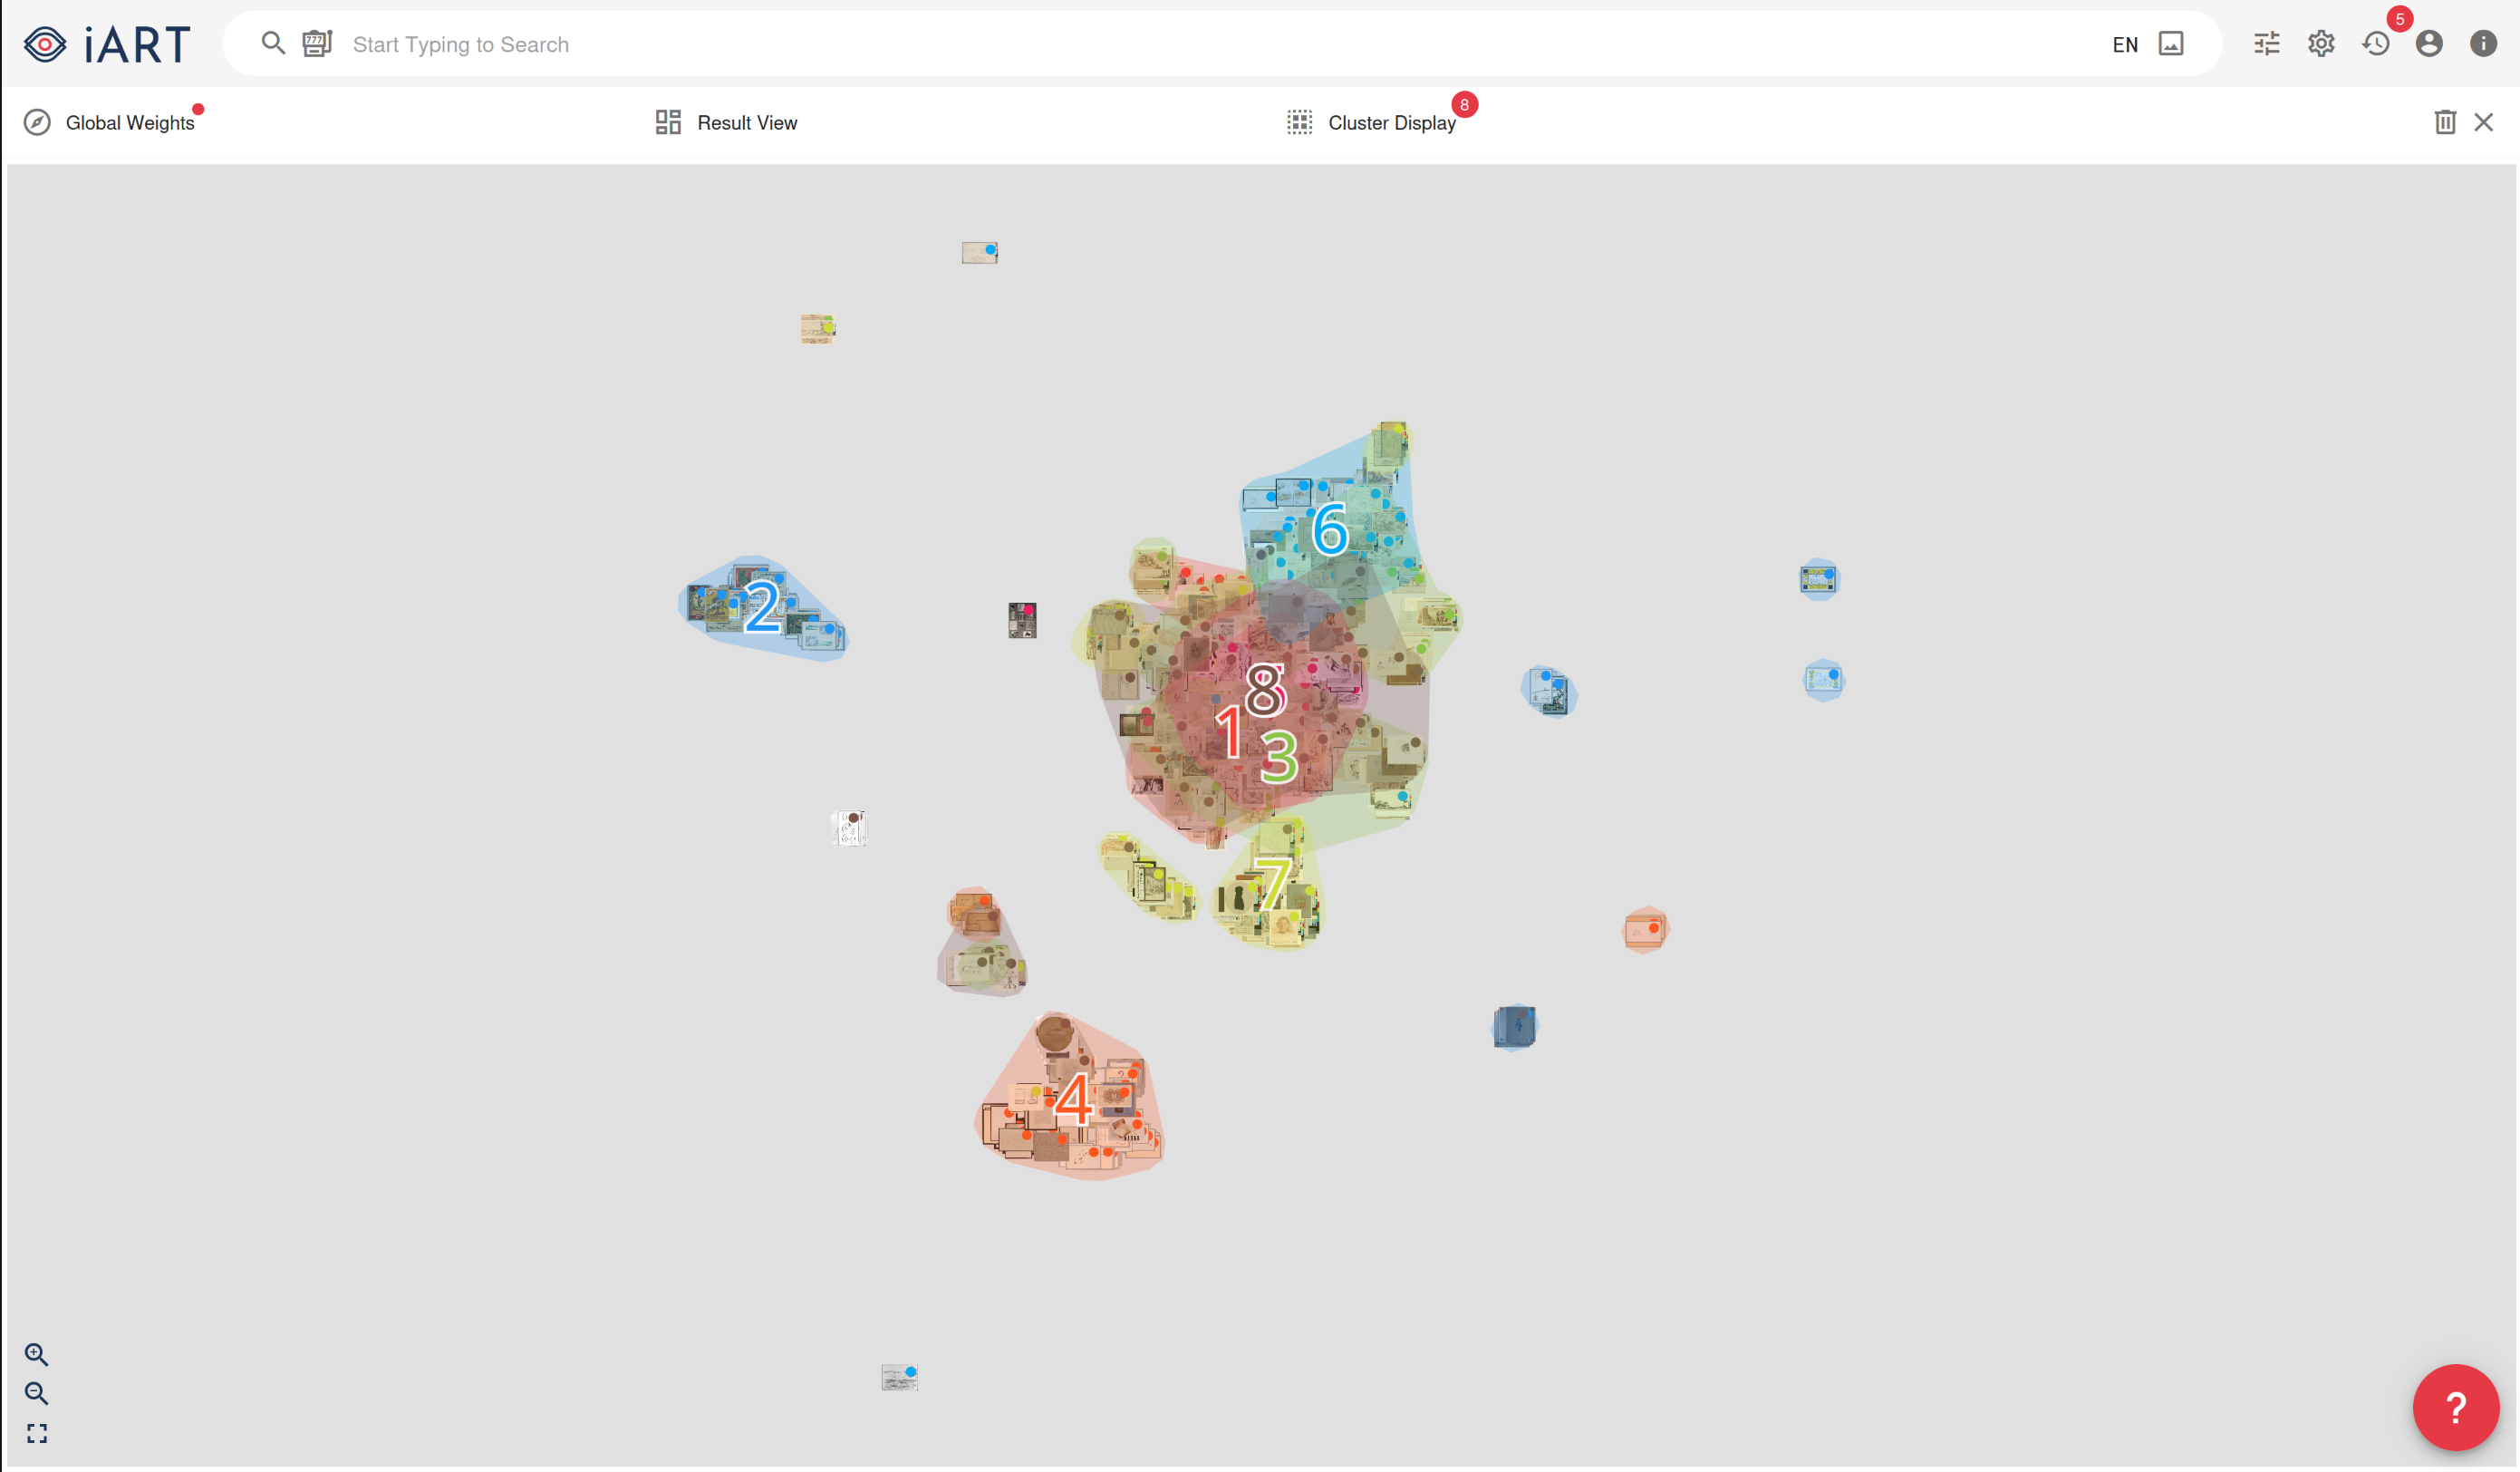
\includegraphics[width=0.8\textwidth]{images/iart_1.png}
	\caption{Visualisation sous forme de \textit{clusters} sur l'interface \textit{iArt}}
	\label{fig:iart_clusters}
\end{figure}

Pour la plateforme \textit{ONiT Explorer}, l'ordre est un peu différent. Lorsque nous faisons une recherche par mot-clé, tous les résultats s'affichent sous une \textit{vue d'ensemble} en mosaïque. Si nous cliquons sur une image, nous obtenons le \textit{détail} de cette dernière avec toutes ses métadonnées. En cliquant sur \textit{More Images (this Book)}, nous avons un \textit{sous-ensemble} contenant toutes les images de l'ouvrage.

\begin{figure}[H]
	\centering
	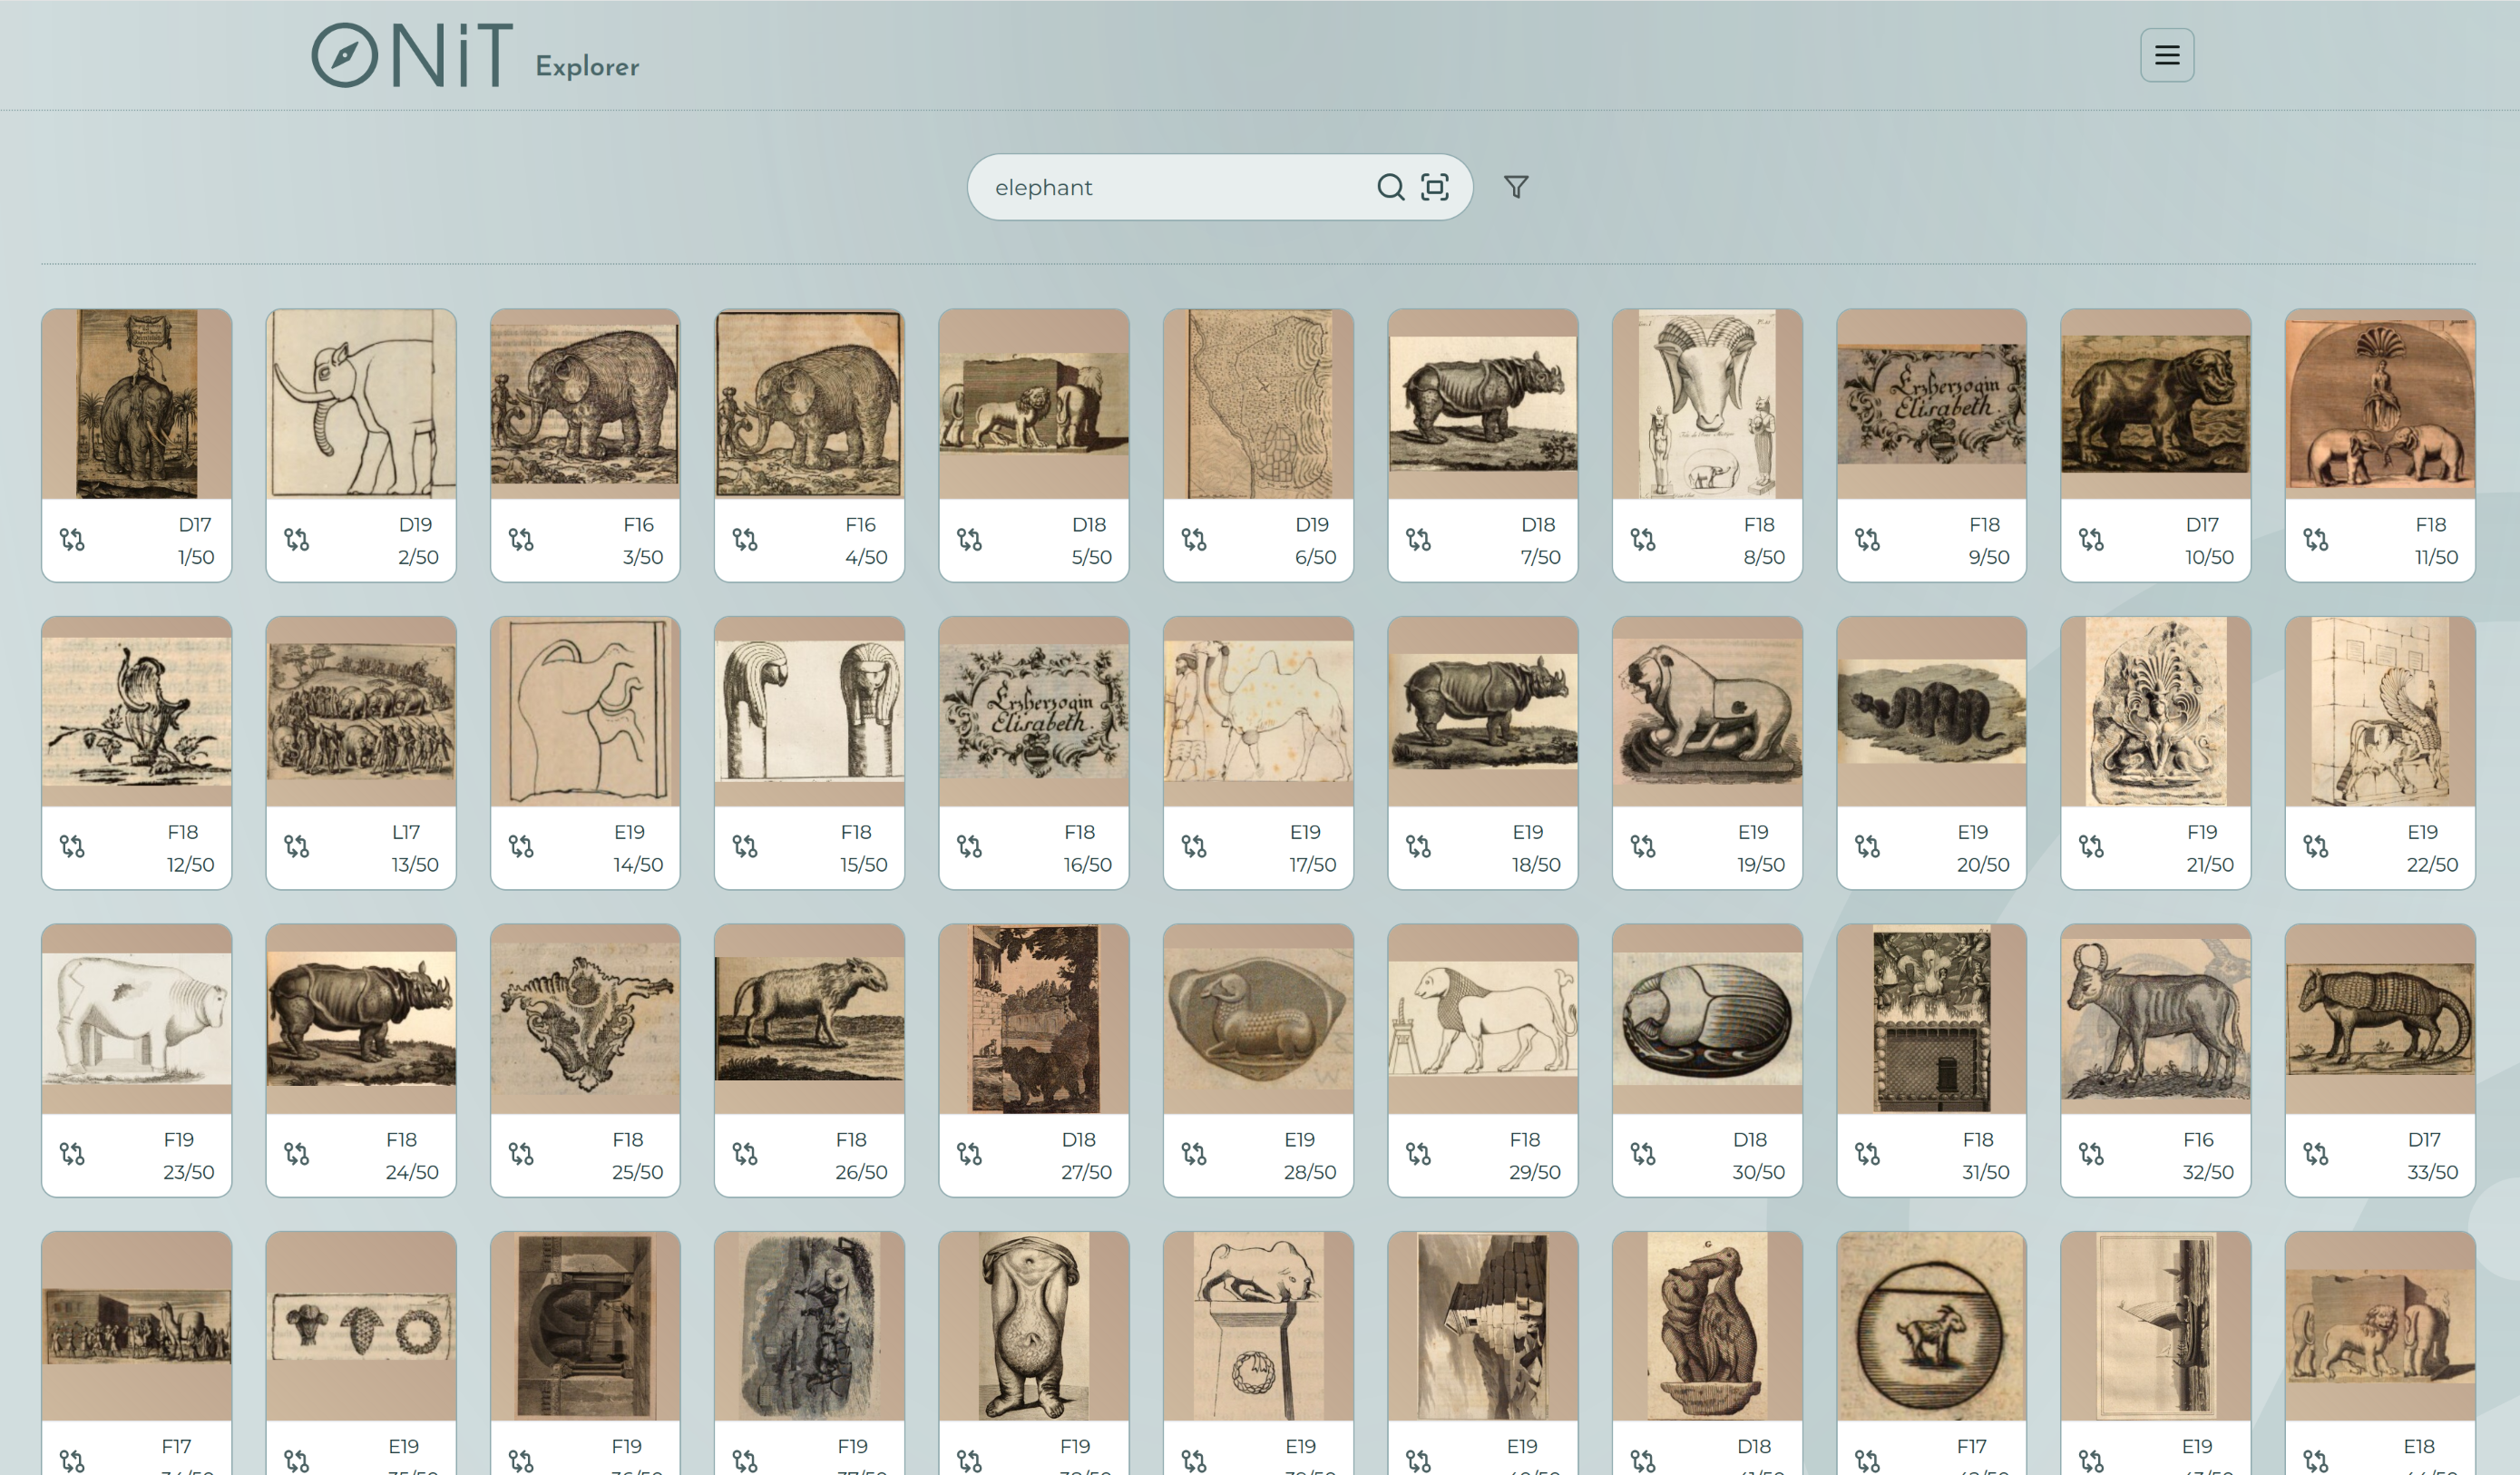
\includegraphics[width=0.8\textwidth]{images/onit_explorer_1.png}
	\caption{L'affichage en mosaïque des résultats de recherche sur la plateforme \textit{ONiT Explorer}}
	\label{fig:onit}
\end{figure}

Dans ces cas de figure, nous pouvons signaler que le type d'affichage favorisé est celui de la mosaïque. 

\subsubsection{Le système de recherche}

La barre de recherche tant décrié par Max Kemman\footcite{kemmanJustGoogleIt2014} et Mitchell Whitelaw\footcite{whitelawGenerousInterfacesDigital2015} est utilisée dans les trois projets mais d'une manière différente. 

Dans la partie exploration du corpus de la plateforme \textit{Explore}, son usage est très limité au profit de la visualisation sous forme de \textit{clusters}. Elle est uniquement utilisée pour filtrer les résultats à l'intérieur de ces derniers.

En ce qui concerne \textit{ONiT Explorer}, la recherche par mot-clé et par image sont les seuls moyens d'entrer dans le corpus. Cela est problématique pour l'utilisateur qui n'est pas familier du corpus et qui n'a pas d'image à comparer. Il s'agit d'un véritable frein pour l'exploration du corpus. Néanmoins, la visualisation des résultats sous la forme d'une mosaïque peut tout de même provoquer la sérendipité si l'utilisateur découvre par hasard une nouvelle image importante pour ses recherches.

\textit{iArt} utilise uniquement une barre de recherche pour l'accès dans son corpus. Cependant, une fonctionnalité \textit{Random Search} permettant de réaliser une recherche aléatoire a été ajoutée à la plateforme. Les images affichées ont une cohérence entre elles. Il est possible de les réunir en \textit{clusters} en utilisant la fonctionnalité \textit{Use 2D Canvas view}. Le sentiment de surprise provoqué par chaque nouvelle recherche est un véritable atout autant pour les \textit{casual users} qui découvrent de nouvelles thématiques que pour les \textit{experts} qui pourraient y puiser des nouvelles idées de projets.

L'usage de \textit{tags} joue également un rôle important dans la recherche de contenu. Il s'agit de mots clés désignant des métadonnées qui permettent de relier différents objets entre-eux. Lorsque nous cliquons sur un tags, toutes les images le possédant s'affichent. Par exemple, si nous utilisant le tag \og chat \fg, toutes les images de la base de données représentant ou ayant un lien avec un chat vont s'afficher.  


\subsubsection{L'interopérabilité}

L'interopérabilité des images dans ce type de projet est un paramètre important à prendre en compte. Sur ces interfaces, il y a de nombreux renvois vers le site de l'institution de conservation lorsque nous consultons un objet. Le standard \gls{iiif} permet la réutilisation des images numérisées par les institutions dans ce type de projet. Il est notamment utilisé dans le projet \textit{Visual Contagion} et dans la plateforme \textit{ONiT Explorer}. Cependant, son usage n'est pas systématique. Le projet \textit{iArt} n'utilise pas ce standard, ce qui peut vite devenir problématique lorsque nous voulons exporter une image en haute résolution.

\subsubsection{La conservation de l'historique}

Pour finir, Shneiderman\footcite{shneidermanEyesHaveIt} conseillait d'intégrer à son interface un moyen de conserver l'historique de l'utilisateur pour ses prochaines visites. Ce critère n'est rempli que par \textit{iArt} qui enregistre automatiquement un historique des recherche réalisées sans avoir besoin de créer un compte. 
